\documentclass{beamer}
\usetheme{Boadilla}
\usepackage{hyperref}
\usepackage{tikz}
\usetikzlibrary{shapes,positioning}
\usepackage{graphicx}
\usepackage{fancyvrb}
\usepackage{multicol}
\usepackage{subfig}
\usepackage{xcolor}
\usepackage{optparams}
\usepackage{xstring}
\usepackage[
    backend=biber, 
    natbib=true,
    style=numeric,
    sorting=none,
    style=verbose-ibid,
]{biblatex}
\addbibresource{citations.bib}
\usepackage{pgfpages}
\definecolor{ao(english)}{rgb}{0.0, 0.5, 0.0}
\definecolor{burgundy}{rgb}{0.5, 0.0, 0.13}
%\setbeameroption{show notes}
%\setbeameroption{show notes on second screen=right}
\setbeameroption{hide notes}

\def\footshortciteintern[#1][#2]#3{%
\ifx#1\empty 
% Nur Autor
\footnote{\citeauthor{#3}, \citeyear{#3}.}
\else
\ifx#2\empty
% Autor und Seite
\footnote{\citeauthor{#3}, \citeyear{#3}, #1.}
\else
% Autor, Seite und vgl.
\expandafter  
\footnote{\citeauthor{#3}, \citetitle{#3}, \citeyear{#3}, \citeurl{#3}.}
\fi
\fi
}
\newcommand*\footshortcite{%
\optparams{\footshortciteintern}{[\empty][\empty]}
}
\newcommand*\footmediumcite{%
\optparams{\footshortciteintern}{[][]}
}


\title{Nonstationary Gabor frames}
\author{Sevag Hanssian}
\date{February 25, 2021}
\institute{MUMT 622, Winter 2021}
\setbeamertemplate{navigation symbols}{}

\begin{document}

\begin{frame}
\maketitle
\end{frame}

\begin{frame}
	\frametitle{Nonstationary Gabor frames}
	\newcounter{year}
	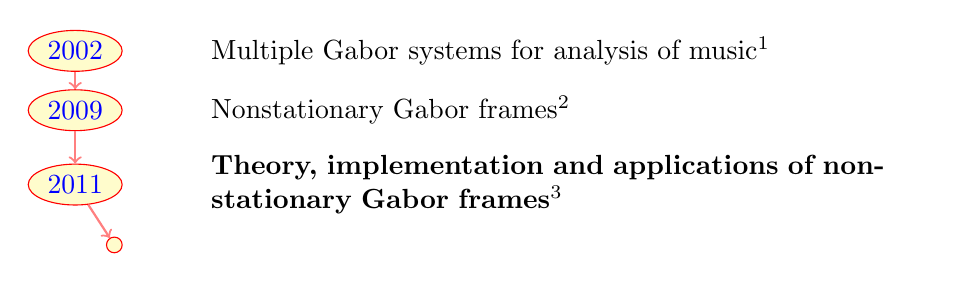
\begin{tikzpicture}[yscale=0.5,%
		   year/.style={draw=red,text=blue,fill=yellow!20,shape=ellipse,inner sep=2pt},
		   description/.style={rectangle,align=left,text width=90mm,anchor=west},
		   timeline/.style={->,thick,red!50}]

	    \foreach \year/\desc [count=\y] in {%
		    2002/Multiple Gabor systems for analysis of music\footnotemark,%
		    2009/Nonstationary Gabor frames\footnotemark,%
		    2011/\textbf{Theory, implementation and applications of nonstationary Gabor frames}\footnotemark,%
	       } { \ifnum\y=1 \node[description](\y){\desc};
		   \else\node[description,below=1ex of \z](\y){\desc};
		   \fi
		   \node[year](y-\y) [left=of \y] {\year};
		   \ifnum\y>1\draw[timeline] (y-\z)-- (y-\y);\fi
		   \global\let\z=\y% for drawing from last node
	       }
	\end{tikzpicture}

	\addtocounter{footnote}{-3} %3=n
	\stepcounter{footnote}\footnotetext{\cite{doerflerphd}}
	\stepcounter{footnote}\footnotetext{\cite{jaillet}}
	\stepcounter{footnote}\footnotetext{\cite{balazs}}
\end{frame}

\note{
	\begin{itemize}
		\item
			Monika D{\"o}rfler's PhD dissertation on gabor, varying TF resolution, music
	\end{itemize}
}

\begin{frame}
	\frametitle{Nonstationary Gabor frames}
	\begin{quote}
		The definition of multiple Gabor frames, which is comprehensively treated in [D{\"o}rfler 2002], provides Gabor frames with analysis techniques with multiple resolutions.\\
		\vspace{0.5em}
		The nonstationary Gabor frames (see [Jaillet 2009], [Balazs 2011] for their definition and implementation)  are a further development; they fully exploit theoretical properties [...] they provide for a class of FFT-based algorithms [...] together with perfect reconstruction formulas\footfullcite{adaptivecqt}
	\end{quote}
\end{frame}

\begin{frame}
	\frametitle{Invertible Constant-Q Transform}
	\newcounter{yeartwo}
	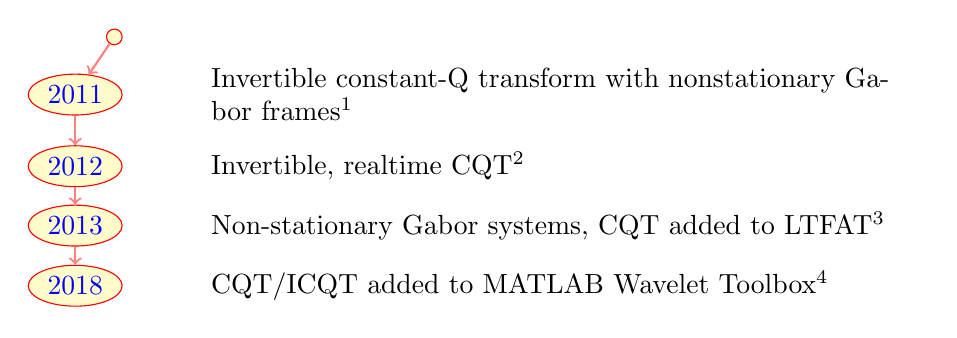
\begin{tikzpicture}[yscale=0.5,%
		   yeartwo/.style={draw=red,text=blue,fill=yellow!20,shape=ellipse,inner sep=2pt},
		   description/.style={rectangle,align=left,text width=90mm,anchor=west},
		   timeline/.style={->,thick,red!50}]

	    \foreach \yeartwo/\desc [count=\y] in {%
		    ,2011/Invertible constant-Q transform with nonstationary Gabor frames\footnotemark,%
		    2012/{Invertible, realtime CQT}\footnotemark,%
		    2013/{Non-stationary Gabor systems, CQT added to LTFAT}\footnotemark,%
		    2018/{CQT/ICQT added to MATLAB Wavelet Toolbox}\footnotemark%
	       } { \ifnum\y=1 \node[description](\y){\desc};
		   \else\node[description,below=1ex of \z](\y){\desc};
		   \fi
		   \node[yeartwo](y-\y) [left=of \y] {\yeartwo};
		   \ifnum\y>1\draw[timeline] (y-\z)-- (y-\y);\fi
		   \global\let\z=\y% for drawing from last node
	       }
	\end{tikzpicture}

	\addtocounter{footnote}{-4} %3=n
	\stepcounter{footnote}\footnotetext{\cite{invertiblecqt}}
	\stepcounter{footnote}\footnotetext{\cite{rtcqt}}
	\stepcounter{footnote}\footnotetext{\cite{ltfat}}
	\stepcounter{footnote}\footnotetext{\cite{matlabcqt}}
\end{frame}

\note{
	\begin{itemize}
		\item
			frame theory led to a serious solution for a practical, invertible CQT
	\end{itemize}
}

\begin{frame}
	\frametitle{Review: Gabor frames}
	Gabor's 1946 ``Theory of Communication''\footfullcite{gabor1946}:
	\begin{enumerate}
		\item
			First introduction of the time-frequency uncertainty principle
		\item
			Proposed that any signal can be chopped up and windowed with Gaussian functions to minimize TF uncertainty
	\end{enumerate}
	    \[ \sigma_{t}\sigma_{f} \ge \frac{1}{4\pi},\qquad\Delta t\Delta f \ge 1 \]
	\begin{figure}
		\vspace{-1.5em}
		\centering
		\subfloat[Max signal localization in TF: rectangles of size $\Delta t\Delta f = 1$]{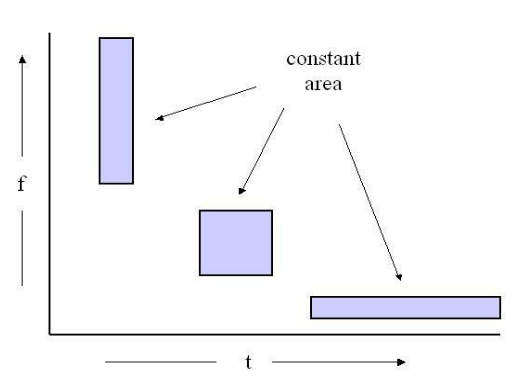
\includegraphics[width=4.5cm]{./tf-resolution.png}}
		\hspace{2.5em}
		\subfloat[Change TF tiling by modifying Gaussian]{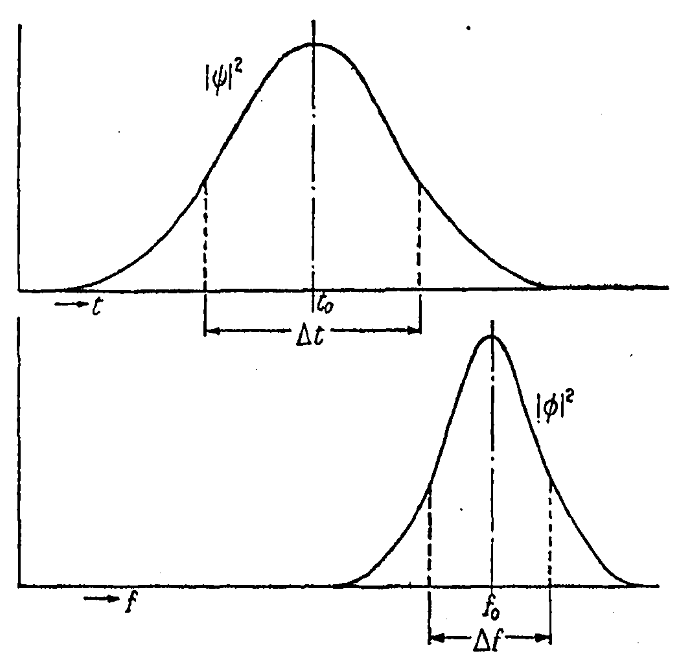
\includegraphics[width=3.5cm]{./gabor4.png}}
	\end{figure}
\end{frame}

\note{
	\begin{itemize}
		\item
			this material builds on the material from my last presentation
		\item
			start with the refresher
		\item
			recall that we are constrained to rectangles of this area
	\end{itemize}
}

\begin{frame}
	\frametitle{Review: fixed TF resolution STFT}
	MATLAB STFT with gausswin (i.e. Gabor transform)
	\begin{figure}
		\centering
		\subfloat[small window (128)]{{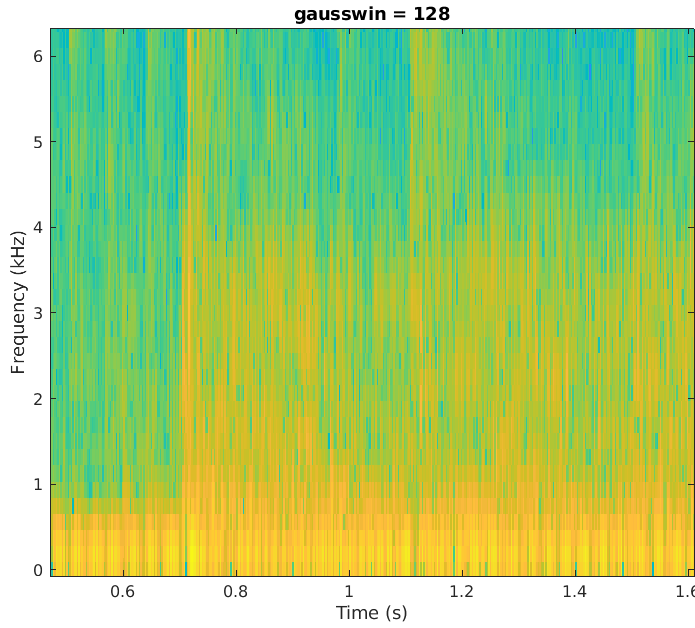
\includegraphics[width=5.04cm]{./gaborstft_small_zoomed.png} }}
		\subfloat[big window (16384)]{{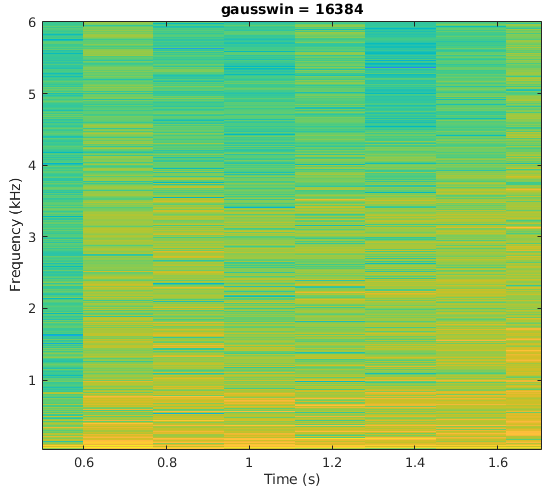
\includegraphics[width=5.1cm]{./gaborstft_big_zoomed.png} }}
		\caption{Good time resolution versus good frequency resolution}
	\end{figure}
\end{frame}

\begin{frame}
	\frametitle{Fixed TF resolution for music}
	\begin{figure}
		\centering
		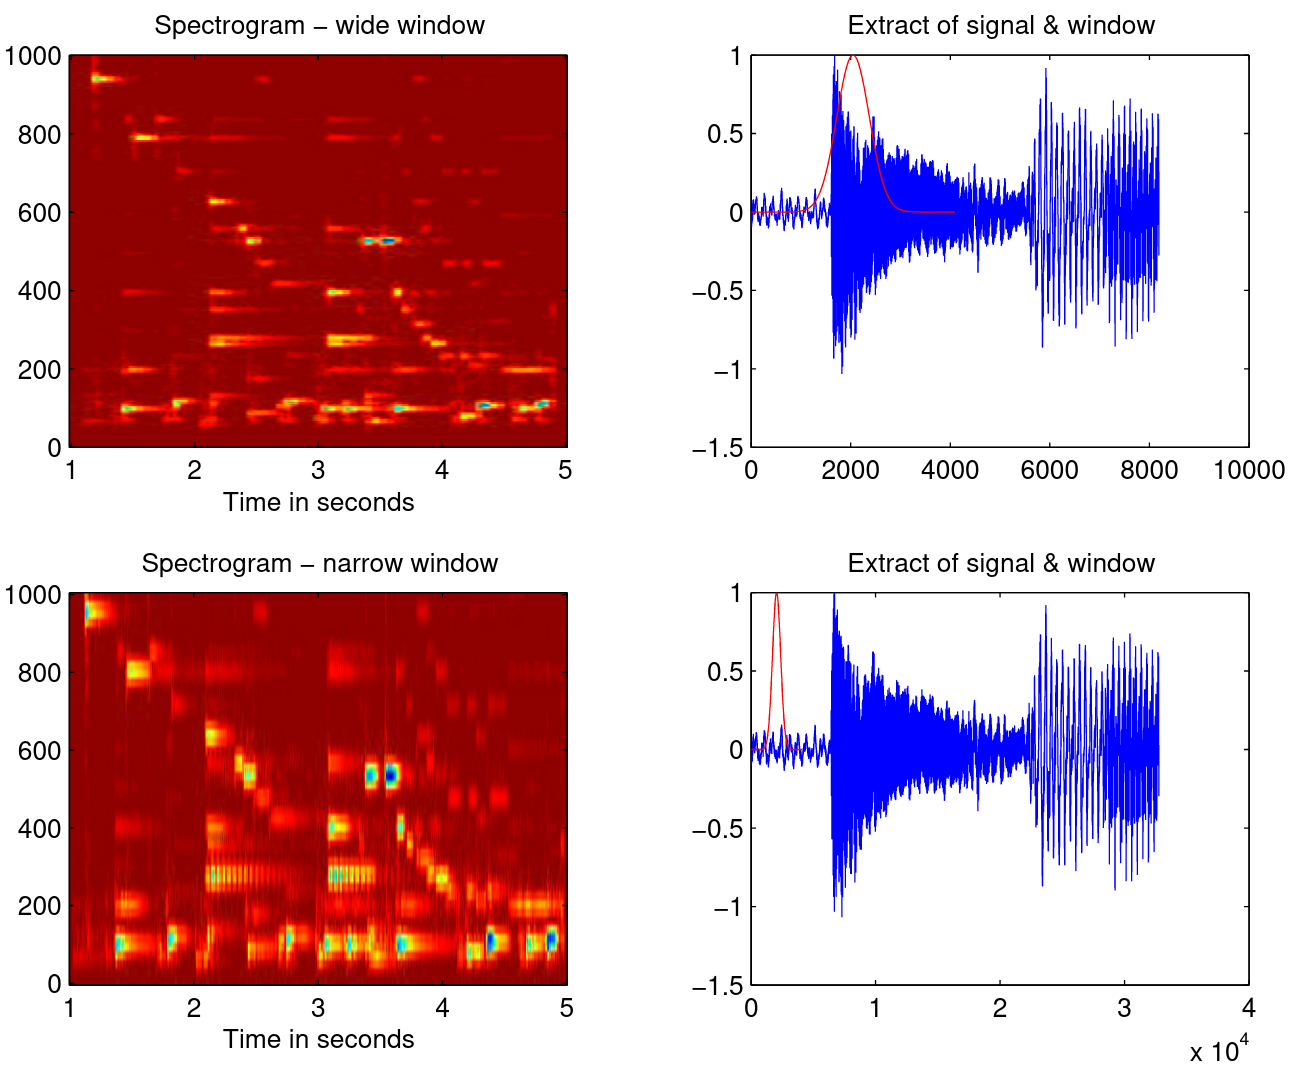
\includegraphics[width=7cm]{./tf_tradeoff_dorfler.png}
		\caption{Two windows for music signal analysis\footshortcite{doerflerphd}}
	\end{figure}
\end{frame}

\begin{frame}
	\frametitle{Stationary Gabor frames}
	In the standard Gabor analysis, same window function (aka Gabor atom, Gabor function) is shifted in time to cover entire signal\footshortcite{adaptivecqt}:
	\[ g_{\tau, \omega}(t) = g(t - \tau)e^{2\pi i t \omega} \]

	\begin{columns}
           \column{0.5\linewidth}
		\begin{quote}
			We will indicate such a frame as \textit{stationary}, since the window used for time-frequency shifts does not change and the time-frequency shifts form a lattice of $a\text{ }x\text{ }b$
		\end{quote}
          \column{0.5\linewidth}
		\hspace{-2em}
		%\vspace{6em}
	    \centering
	     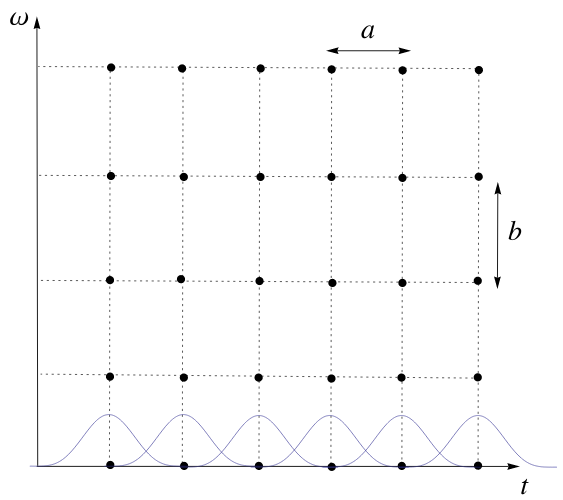
\includegraphics[width=4cm]{stationarygabor.png}
        \end{columns} 
\end{frame}

\note{
	\begin{itemize}
		\item
			Last presentation, I didn't call it stationary - only ``gabor frame'' alone
		\item
			until the non-stationary variant was created, there was no need to call the original stationary
	\end{itemize}
}

\begin{frame}
	\frametitle{Early CQT: musical motivation}
		Constant-Q transform for music analysis\footfullcite{jbrown}, \footfullcite{msp}:
		\begin{enumerate}
			\item
				Harmonics of the fundamental have consistent spacing in the log scale -- the constant pattern\\
				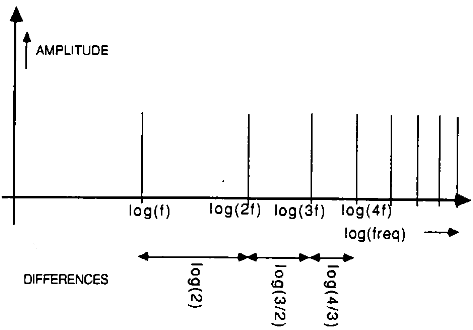
\includegraphics[height=3cm]{./logharmonic.png}
			\item
				Log-frequency spectra, demonstrating the constant pattern for harmonics, would be more useful in musical tasks
		\end{enumerate}
\end{frame}

\note{
	\begin{itemize}
		\item
			judith brown, MSP (of miller s puckette fame)
		\item
			constant-Q transform was known about before Gabor frames - like i discussed with prof
		\item
			tasks such as instrument identification by timbre, etc.
		\item
			also lines up with pitch perception as pattern recognition
	\end{itemize}
}

\begin{frame}
	\frametitle{Violin: DFT vs. CQT}
	\begin{figure}
		\vspace{-1em}
		\centering
		\subfloat[Discrete Fourier Transform]{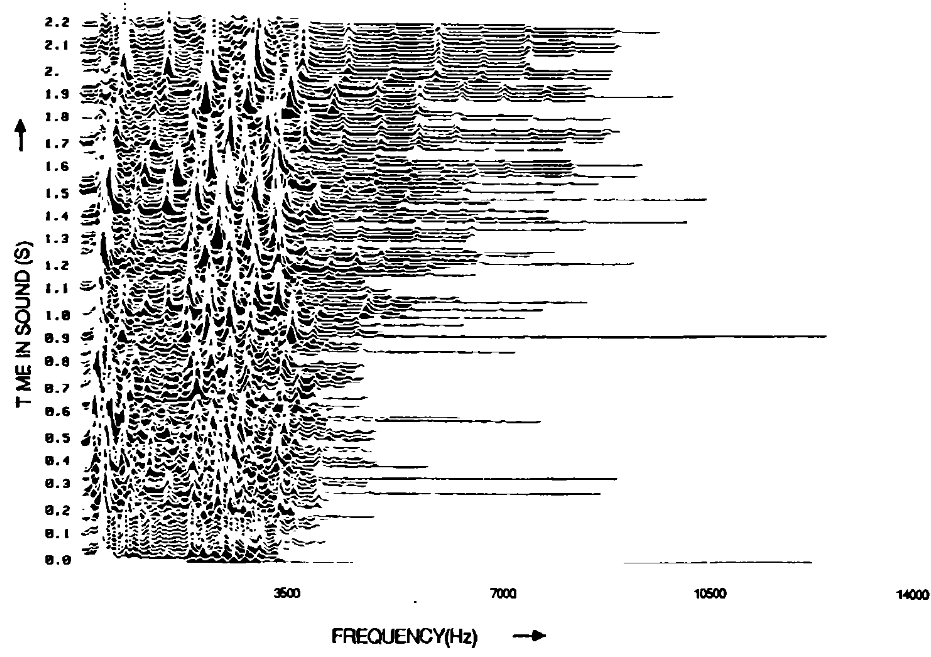
\includegraphics[height=3.75cm]{./violindft.png}}
		\subfloat[Constant Q transform]{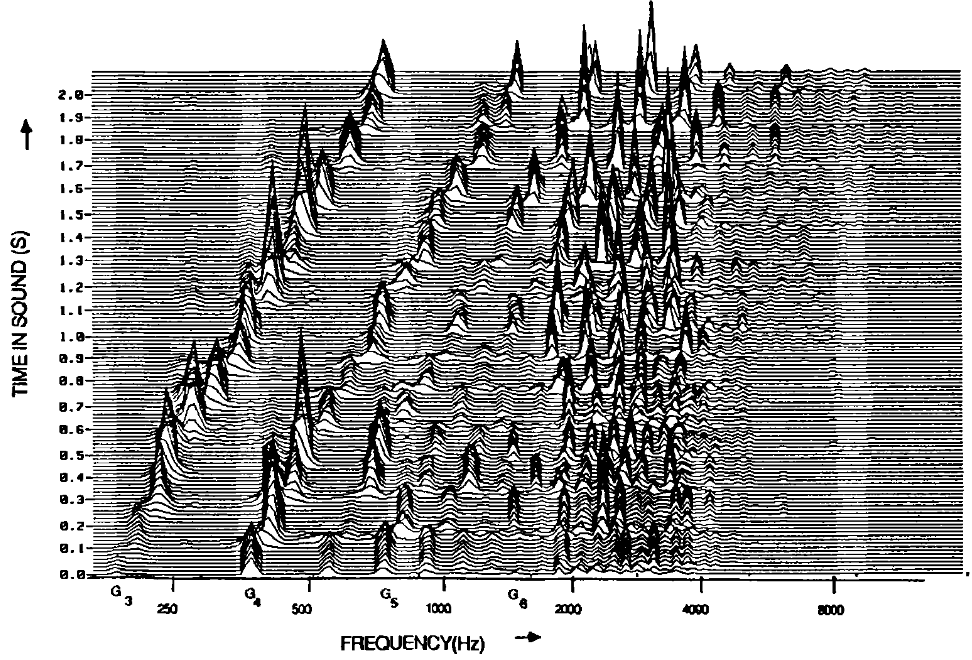
\includegraphics[height=3.75cm]{./violincqt.png}}
		\caption{Violin playing diatonic scale, $G_{3} \text{(196Hz)} - G_{5} \text{(784Hz)}$\footshortcite{jbrown}}
	\end{figure}
\end{frame}

\note{
	\begin{itemize}
		\item
			Not explicitly named as an STFT but we know it is
		\item
			we can see note changes clearly, the fundamental, and even the formant in 3000hz region
	\end{itemize}
}

\begin{frame}
	\frametitle{Constant-Q Transform}
	``Constant ratio of frequency to frequency resolution'': $\frac{f}{\delta f} = Q$
	\begin{figure}
		\vspace{-1em}
		\centering
		\subfloat[Properties of DFT, CQT]{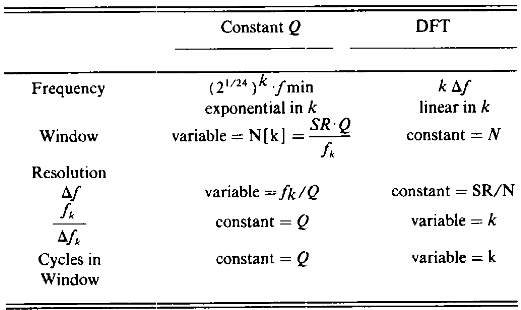
\includegraphics[height=3.5cm]{./dftvcqt.png}}
		\subfloat[Window sizes for CQT]{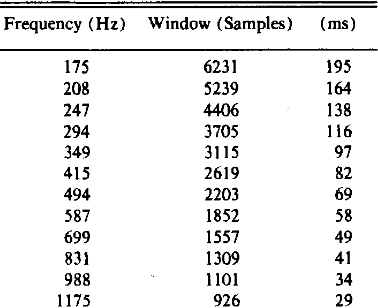
\includegraphics[height=3.5cm]{./qwindowchanges.png}}
	\end{figure}
	Computed with windowed DFT where window changes with frequency to maintain Constant-Q\footshortcite{jbrown} -- \textbf{non-invertible!}:
	\[ \text{window len } N[k] = \frac{f_{s}}{f_{k}}Q, W[k, n] = \alpha + (1 - \alpha)\cos(\frac{2\pi n}{N[k]}) \]
\end{frame}

\note{
	\begin{itemize}
		\item
			meanwhile the linear spacing of conventional DFT leads to a pattern that varies with the harmonic -- making it harder to identify 
		\item
			in linear DFT, pattern of harmonic spacing changes with frequency
	\end{itemize}
}

\begin{frame}
	\frametitle{Multiple Gabor systems: musical motivation}
	\begin{quote}
		In the case of music signals, for example, transients are important for several reasons. They give important cues for onset timing, and they carry information about instrument timbre. As another example, in low-frequency regions, very fine frequency resolution is required, because notes in this region lay the harmonic basis, musically speaking.\\
		\vspace{0.4em}
		In order to achieve a setting adapted to music as discussed above, it will be necessary to use wider windows with good frequency concentration in low-frequency regions, whereas in the high-pass regions, where mainly transients and broadband signals components occur, rather short windows, which don't have to be very localised in frequency, will be of use \footshortcite{doerflerphd}
	\end{quote}
\end{frame}

\note{
	\begin{itemize}
		\item
			similar motivation, except Dorfler et all are using this motivation to drive mathematical theory
		\item
			the lack of theory didn't affect the evolution, or desire, for the CQT
	\end{itemize}
}

\begin{frame}
	\frametitle{Multi-window Gabor dictionary}
	Stationary Gabor atom, where $a$ and $b$ are TF shift parameters:
	\[ g_{m,n}(t) = g(t - na)e^{j2\pi m b t},\qquad m,n \in \mathbb{Z} \]
	\[ f(t) = \sum_{m,n \in \mathbb{Z}}c_{m,n}g_{m,n}(t) \]
	Use $R$ different windows, where $a_{r}$ and $b_{r}$ are TF shift parameters for each distinct window:
	\[ g_{m,n}^{r}(t) = g(t - na_{r})e^{j2\pi m b_{r} t},\qquad m,n \in \mathbb{Z} \]
	\[ f(t) = \sum_{r=0}^{R-1}\sum_{m,n \in \mathbb{Z}}c^{r}_{m,n}g^{r}_{m,n}(t) \]
\end{frame}

\note{
	\begin{itemize}
		\item
			f = signal, constructed from time-frequency shifts of gabor atoms
	\end{itemize}
}

\begin{frame}
	\frametitle{Example: multiple STFTs}
	\begin{figure}
		\centering
		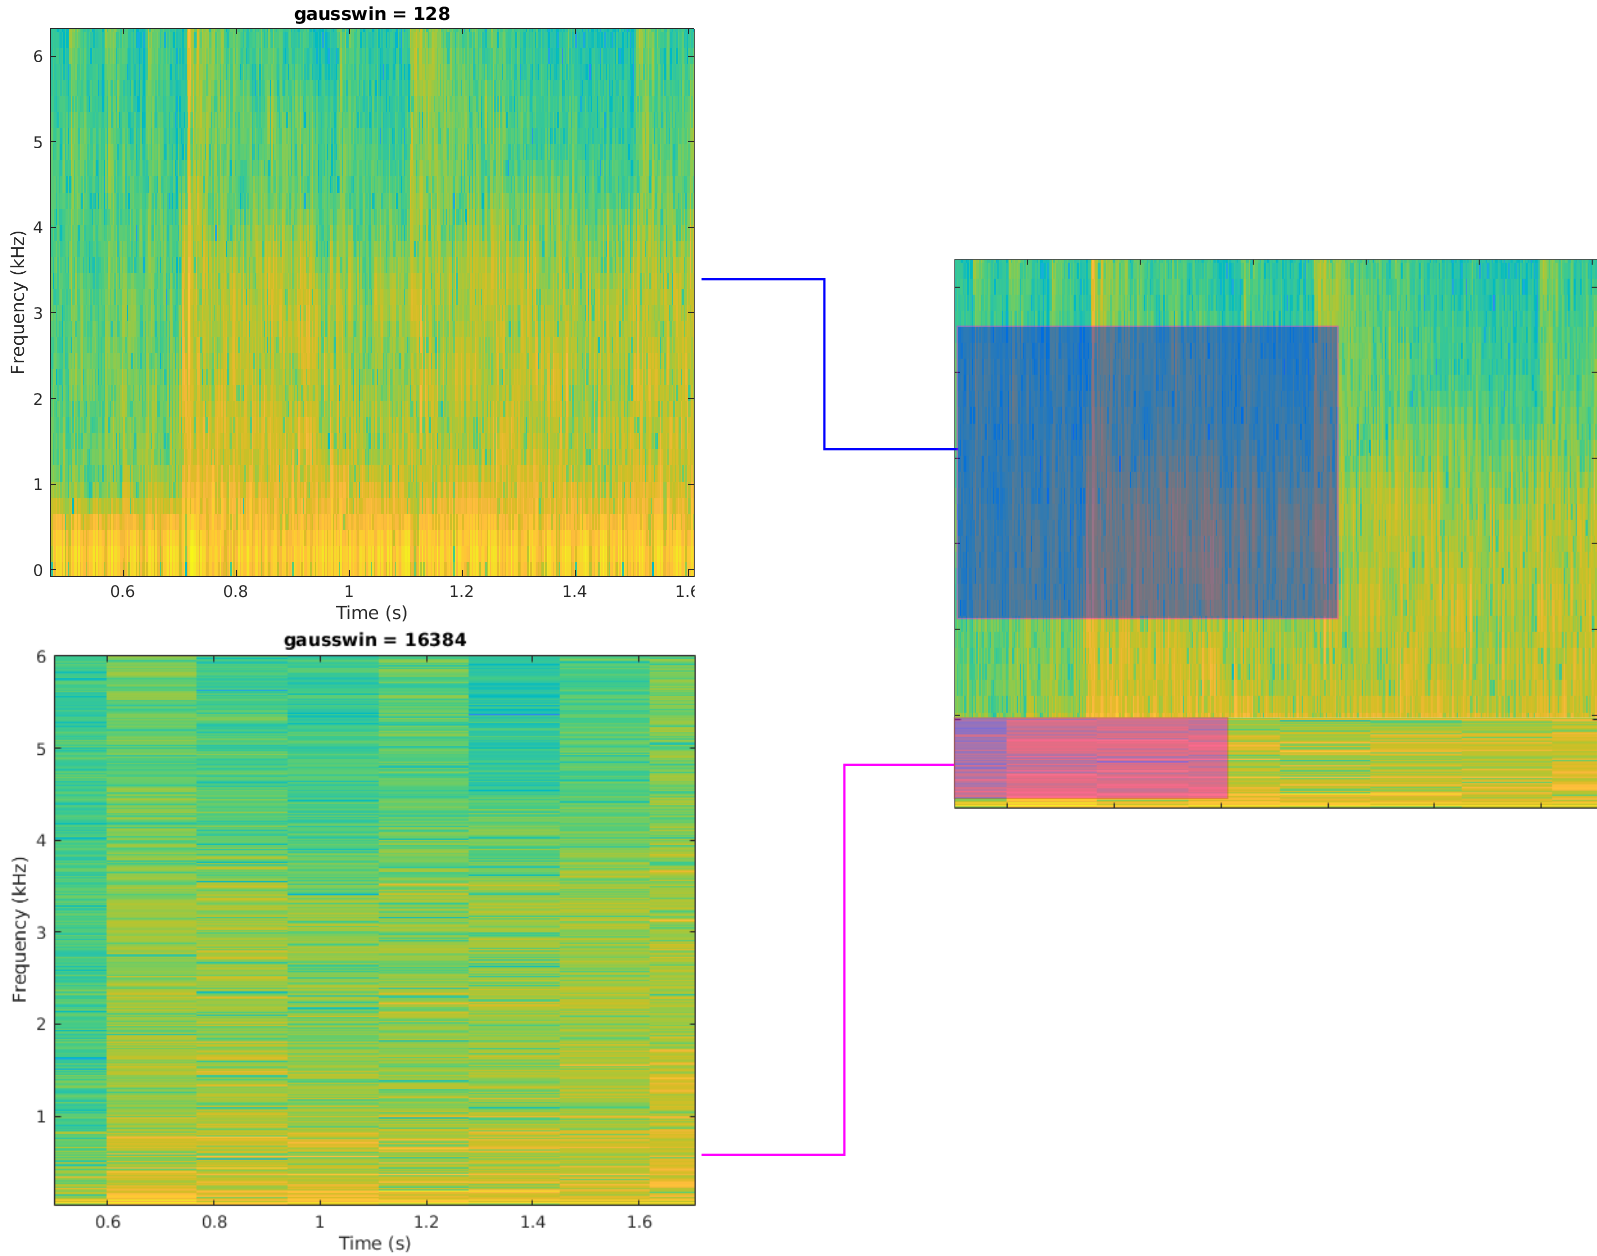
\includegraphics[width=8cm]{./naivemixedstft.png}
		\caption{Multiple ($R = 2$) Gabor dictionaries with stationary frames}
	\end{figure}
\end{frame}

\note{
	\begin{itemize}
		\item
			fulfills musical requirements (good frequency resolution in low-frequency region, good time resolution in high-frequency region)
		\item
			highly redundant, overcomplete
		\item
			choose appropriate window STFT for each region of interest
		\item
			According to the multi-window approach, the dictionary will have high redundancy as it is basically the combination of R complete Gabor dictionaries. Due to the structure of audio signals, it is an appealing idea to reduce this highly redundant dictionary to fit to the special characteristics of these signals.
	\end{itemize}
}

\begin{frame}
	\frametitle{Nonstationary Gabor frame -- resolution changing over time}
	Stationary Gabor atom, where $a$ and $b$ are TF shift parameters:
	\[ g_{m,n}(t) = g(t - na)e^{j2\pi m b t},\qquad m,n \in \mathbb{Z} \]
	Nonstationary Gabor atom from a set of functions $\{g_{n}\}$ and a fixed frequency sampling step $b_{n}$\footshortcite{balazs}:
	\[ g_{m,n}(t) = g_{n}(t)e^{j2\pi m b_{n}t},\qquad m,n \in \mathbb{Z} \]
	We get back classic nonstationary Gabor frame by setting:
	\[ g_{n}(t) = g(t - na) \text{ for a fixed time constant } a, b_{n} = b \forall n \]
\end{frame}

\begin{frame}
	\frametitle{Nonstationary Gabor frame -- resolution changing over time}
	\begin{quote}
		[...] the functions $\{g_{n}\}$ are well-localized and centered around time-points $a_{n}$. This is similar to the standard Gabor scheme [...] with the possibility to vary the window $g_{n}$ for each position $a_{n}$. Thus, sampling of the time-frequency plane is done on a grid which is irregular over time, but regular over frequency at each temporal position.\footshortcite{balazs}
	\end{quote}
	\begin{figure}
		\centering
		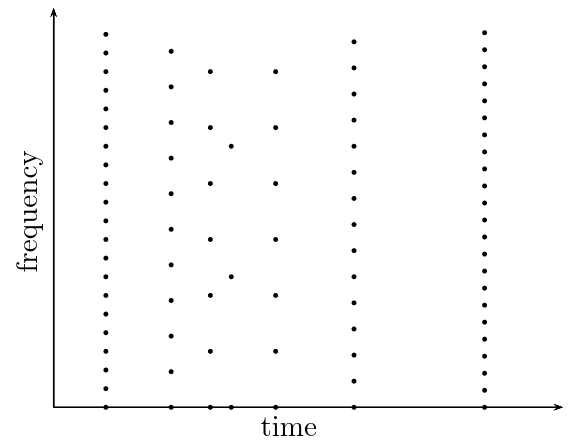
\includegraphics[width=5cm]{./irregulartime.png}
		\caption{Irregular TF sampling grid}
	\end{figure}
\end{frame}

\begin{frame}
	\frametitle{Nonstationary Gabor frame -- resolution changing over frequency}
	Stationary Gabor atom, where $a$ and $b$ are TF shift parameters:
	\[ g_{m,n}(t) = g(t - na)e^{j2\pi m b t},\qquad m,n \in \mathbb{Z} \]
	Nonstationary Gabor atom from a family of functions $\{h_{m}\}$ and a fixed time sampling step $a_{m}$\footshortcite{balazs}:
	\[ h_{m,n}(t) = h_{m}(t - na_{m}),\qquad m,n \in \mathbb{Z} \]
	We get back classic nonstationary Gabor frame by setting:
	\[ h_{m}(t - na_{m}) = g(t - na)e^{j2\pi m b t} \text{ for a fixed frequency constant } b, a_{m} = a \forall m \]
\end{frame}

\begin{frame}
	\frametitle{Nonstationary Gabor frame -- resolution changing over frequency}
	\begin{quote}
		In practice we will choose each function $h_{m}$ as a well-localized band-pass function with center frequency $b_{n}$\footshortcite{balazs}
	\end{quote}
	\begin{figure}
		\centering
		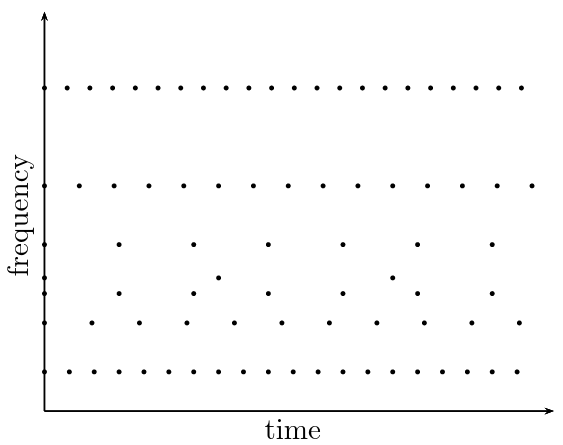
\includegraphics[width=5cm]{./irregularfrequency.png}
		\caption{Irregular TF sampling grid}
	\end{figure}
\end{frame}

\begin{frame}
	\frametitle{Nonstationary Gabor frame construction}
	Construction of painless nonstationary Gabor frames relies on three properties of the windows and time-frequency shift parameters used\footshortcite{balazs}:
	\begin{itemize}
		\item
			The signal $f$ of interest is localized at time- (or frequency-) positions $n$ by means of multiplication with a compactly supported (or limited bandwidth, respectively) window function $g_{n}$
		\item
			The Fourier transform is applied on the localized pieces $f \cdot g_{n}$. The resulting spectra are sampled densely enough in order to perfectly re-construct $f \cdot g_{n}$ from these samples
		\item
			Adjacent windows overlap to avoid loss of information. At the same time, unnecessary overlap is undesirable. We assume that $0 < A \le \sum_{n \in \mathbb{Z}}|g_{n}(t)|^{2} \le B < \infty$, a.e., for some positive A and B
	\end{itemize}
	These requirements lead to invertibility of the frame operator and therefore to perfect reconstruction.
\end{frame}

\note{
	\begin{itemize}
		\item
			a.e. = almost everywhere
		\item
			 Moreover, the frame operator is diagonal and its inversion is straight-forward. Further, the canonical dual frame has the same structure as the original one. Because of these pleasant consequences following from the three above-mentioned requirements, the frames satisfying all of them will be called painless nonstationary Gabor frames and we refer to this situation as the painless case
	\end{itemize}
}

\begin{frame}
	\frametitle{Discrete nonstationary Gabor frame numerical complexity}
	Discrete nonstationary Gabor frame in discrete time (analogous to continuous time)\footshortcite{balazs}:
	\[ g_{m,n}[k] = g_{n}[k] \cdot e^{\frac{j2\pi m b_{n}k}{L}} = g_{n}[k] \cdot W_{L}^{mb_{n}k} \]
	\[ n = 0, ..., N-1, m = 0, ..., M_{n}-1, k = 0, ..., L = 1 \]\\
	\vspace{1em}
	Nonstationary Gabor coefficients are given by an FFT of length $M_{n}$ for each window $g_{n}$ with a signal of length $L_{n}$\\
	\vspace{1em}
	\begin{enumerate}
		\item
			Windowing: $L_{n}$ operations for the $n$th window
		\item
			FFT: $O(M_{n} \cdot \log(M_{n}))$ for the $n$th window
		\item
			Total: $O(N \cdot (M \log(M)))$ for $N$ windows
	\end{enumerate}
\end{frame}

\begin{frame}
	\frametitle{Result of nonstationary Gabor decomposition}
	\begin{figure}
		\centering
		\subfloat[Stationary Gabor decomposition for 2 different window sizes]{{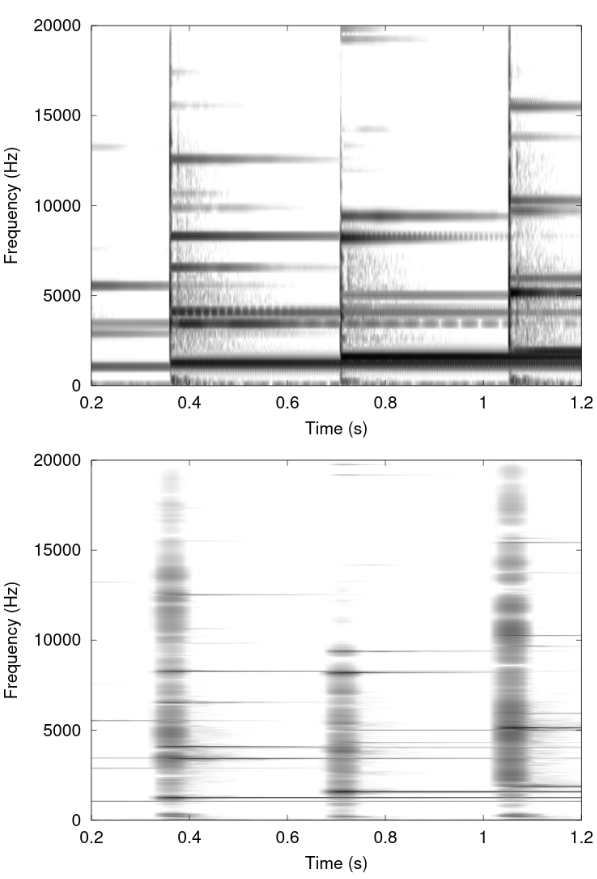
\includegraphics[width=3.5cm]{./tf_tradeoff_balasz1.png} }}
		\hspace{0.5em}
		\subfloat[Nonstationary Gabor decomposition]{{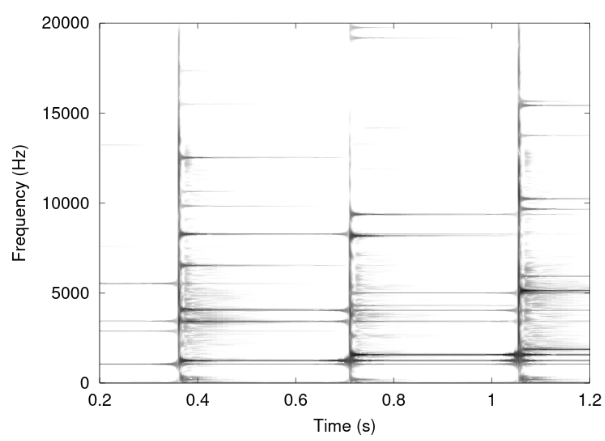
\includegraphics[width=3.5cm]{./tf_tradeoff_balasz2.png} }}
		\caption{Best of both worlds in a single representation\footshortcite{jaillet} (glockpenspeil signal)}
	\end{figure}
\end{frame}

\note{
	\begin{itemize}
		\item
			i skipped many details proving the invertibility, tightness, minimizing redundancy
	\end{itemize}
}

\begin{frame}
	\frametitle{Applications of NSGT: invertible CQT}
	\begin{itemize}
		\item
			Original CQT\footshortcite{jbrown} is non-invertible and computationally intensive
		\item
			Modification\footshortcite{msp} improves computational efficiency
		\item
			Previous approach by \citet{klapuri} has an RMS error of $10^{-3}$ from approximate reconstruction (used in librosa)
			\begin{quote}
			The lack of perfect invertibility prevents the convenient modification of CQT coefficients with subsequent resynthesis required in complex music processing tasks such as masking or transposition.
			\end{quote}
		\item
			NSGT CQT is faster and perfectly invertible; adaptive resolution in frequency results in desired constant Q-factor
		\item
			Drop-in replacement for STFT in music algorithms
	\end{itemize}
\end{frame}

\note{
	\begin{itemize}
		\item
			so first its interesting that even today the outcomes of this paper are yet to spread - librosa currently has an unusable CQT!
		\item
			the invertible CQT is amazing because it's basically a drop-in replacement of the STFT - you can do time-frequency masking, magnitude/power "spectrogram" equivalent - benefit automatically from the musical considerations baked into the CQT
		\item
			talk about fitzgerald source separation
	\end{itemize}
}

\end{document}
